%%%%
\documentclass[10pt]{report}
\usepackage{graphicx,color,epsfig,psfig,subfigure}
\usepackage{amsmath,amsfonts,amssymb}
\usepackage{bm}
\pagestyle{empty}
\begin{document}
\begin{picture}(0,0)%
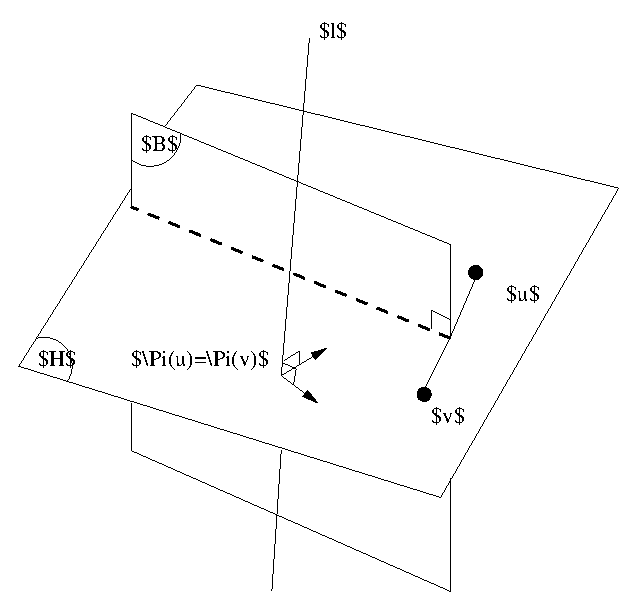
\includegraphics{preuve_bis.pstex}%
\end{picture}%
\setlength{\unitlength}{3947sp}%
%
\begingroup\makeatletter\ifx\SetFigFont\undefined%
\gdef\SetFigFont#1#2#3#4#5{%
  \reset@font\fontsize{#1}{#2pt}%
  \fontfamily{#3}\fontseries{#4}\fontshape{#5}%
  \selectfont}%
\fi\endgroup%
\begin{picture}(4824,4602)(1489,-4123)
\put(3901,314){\makebox(0,0)[lb]{\smash{\SetFigFont{12}{14.4}{\familydefault}{\mddefault}{\updefault}{\color[rgb]{0,0,0}$l$}%
}}}
\put(5401,-1786){\makebox(0,0)[lb]{\smash{\SetFigFont{12}{14.4}{\familydefault}{\mddefault}{\updefault}{\color[rgb]{0,0,0}$u$}%
}}}
\put(4801,-2761){\makebox(0,0)[lb]{\smash{\SetFigFont{12}{14.4}{\familydefault}{\mddefault}{\updefault}{\color[rgb]{0,0,0}$v$}%
}}}
\put(1651,-2311){\makebox(0,0)[lb]{\smash{\SetFigFont{12}{14.4}{\familydefault}{\mddefault}{\updefault}{\color[rgb]{0,0,0}$H$}%
}}}
\put(2476,-586){\makebox(0,0)[lb]{\smash{\SetFigFont{12}{14.4}{\familydefault}{\mddefault}{\updefault}{\color[rgb]{0,0,0}$B$}%
}}}
\put(2401,-2311){\makebox(0,0)[lb]{\smash{\SetFigFont{12}{14.4}{\familydefault}{\mddefault}{\updefault}{\color[rgb]{0,0,0}$\Pi(u)=\Pi(v)$}%
}}}
\end{picture}
\end{document}
